\documentclass[12pt, twoside]{article}
\usepackage[letterpaper, margin=1in, headsep=0.5in]{geometry}
\usepackage[english]{babel}
\usepackage[utf8]{inputenc}
\usepackage{amsmath}
\usepackage{amsfonts}
\usepackage{amssymb}
\usepackage{tikz}
\usepackage{yhmath}
%\usetikzlibrary{quotes, angles}

\usepackage{graphicx}
\usepackage{enumitem}
\usepackage{multicol}

\usepackage{fancyhdr}
\pagestyle{fancy}
\fancyhf{}
\renewcommand{\headrulewidth}{0pt} % disable the underline of the header

\fancyhead[RE]{\thepage}
\fancyhead[RO]{\thepage \\ Name: \hspace{3cm}}
\fancyhead[L]{BECA / Dr. Huson / 10th Grade Geometry\\* 11 June 2019}

\begin{document}
\subsubsection*{13.8 Homework: Circle situations \& trigonometry}
 \begin{enumerate}

  \item Circle $O$ has a radius $AO=7$, as shown below, and arc measure $m \wideparen{AB}=80^\circ$.
     \begin{center}
     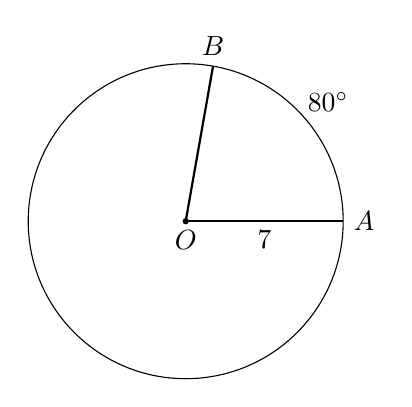
\begin{tikzpicture}[scale=.4]
       \draw (0,0) circle[radius=5];
       \draw [thick]
       (0:5) node[right] {$A$}--(0,0);
       \draw [thick] (0,0)--(80:5) node[above] {$B$};
       \fill (0,0) circle[radius=0.1] node[below]{$O$};
       \draw (40:5.9) node{$80^\circ$};
       \draw (0:2.5) node[below]{$7$};
       %\draw (75:1.8) node[above] {$C$};
       %\draw (290:5) node[below] {$D$};
     \end{tikzpicture}
   \end{center}
   \begin{enumerate}
     \item Find the $m \angle AOB$. \vspace{1cm}
     \item Find the length of the arc $\wideparen{AB}$. \vspace{2.5cm}
     \item Find the area of the sector $AOB$. \vspace{2.5cm}
   \end{enumerate}

   \item Given circle $O$ with points $P$ and $Q$ on the circle. $m\angle POQ=110$. Find $m\angle P$.\\[1cm]
       %\hspace{1cm} Given the line  $l$ and point $P$.
       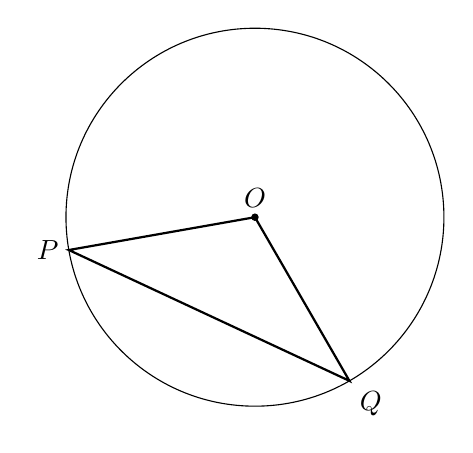
\begin{tikzpicture}[scale=0.8]
         %\draw [-, thick] (-6,0) node[left]{$A$}--(0,0);
         \draw  (0,0) circle [radius=3] node[above]{$O$};
         \draw [-, thick] (190:3) node[left]{$P$}--(0,0)
           --(300:3) node[below right]{$Q$}--cycle;
         %\node at (8.5,-0.4){$l$};
         \draw [fill] (0,0) circle [radius=0.05];
       \end{tikzpicture} %\vspace{3cm}

\newpage
\item Express each value to \emph{the nearest tenth}.  \vspace{0.5cm}
  \begin{multicols}{2}
    \begin{enumerate}
      \item $\tan 76^\circ = $ \vspace{0.5cm}
      \item $\cos 36^\circ =$
      \item $\tan^{-1} 1.73 = $ \vspace{0.5cm}
      \item $\sin^{-1} 0.5 =$
    \end{enumerate}
  \end{multicols}

  \item $\triangle ABC$ has sides of length $BC=6$, $AC=8$, and $AB=10$ as shown, with $m\angle C=90^\circ$. \vspace{0.5cm}
  \begin{multicols}{2}
      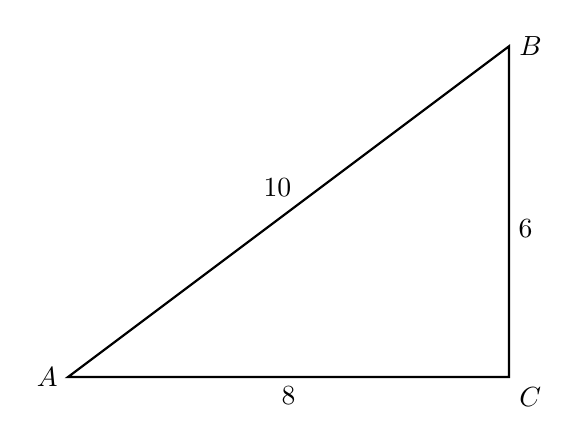
\begin{tikzpicture}[scale=0.7]
        \draw [thick]
        (0,0)node[left]{$A$}--
        (8,0)node[below right]{$C$}--
        (8,6)node[right]{$B$}--cycle;
        \node at (4,0)[below]{$8$};
        \node at (8,2.7)[right]{$6$};
        \node at (3.8,3.1)[above]{$10$};
      \end{tikzpicture}
        \begin{enumerate}
          \item Find $\tan A =$ \vspace{0.75cm}
          \item Find $\cos A =$ \vspace{0.75cm}
          \item Find $\sin B =$ \vspace{0.75cm}
          \item Find $m\angle A =$ \vspace{0.75cm}
      \end{enumerate}
    \end{multicols} \vspace{0.5cm}

  \item Right $\triangle ABC$ is drawn with point $D$ on $\overline{AC}$. $m\angle BAC=40^\circ$, $m\angle BDC=80^\circ$, $m\angle C=90^\circ$, and $AC=10$. \\[0.5cm]
  Find $BC$. Now find $CD$ and $AD$. \vspace{0.5cm}
      \begin{flushright}
        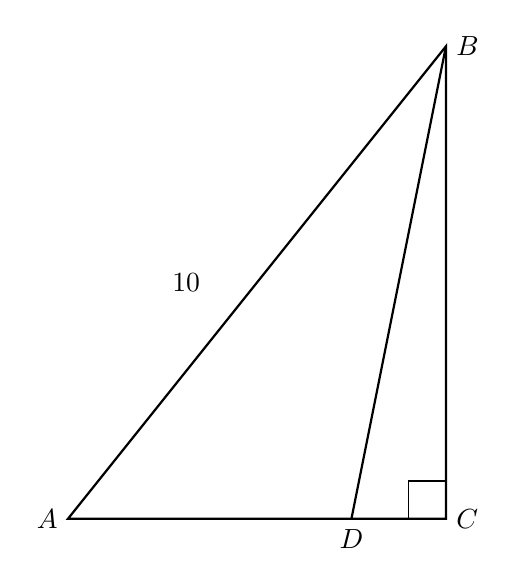
\begin{tikzpicture}[scale=0.6]
          \draw [thick] (-8,0)node[left]{$A$}
          --(0,0)node[right]{$C$}
          --(0,10)node[right]{$B$}--cycle;
          %\draw (0,0) circle [radius=5] node[below]{$O$};
          \draw [thick] (-2,0)node[below]{$D$}--(0,10);
          \draw (0,0) ++(-180:0.8)-- ++(90:0.8)-- +(0:0.8);
          \node at (-5,5)[left]{10};
        \end{tikzpicture}
     \end{flushright}%\vspace{5cm}

\newpage
  \item In a right triangle, the acute angles have the relationship $\sin (x)=\cos(60)$.\\[0.25cm]
    What is the value of $x$? \vspace{2cm}

  \item If $\sin (5x-7)^\circ = \cos(3x+17)^\circ$, what is the value of $x$? \vspace{5cm}

  \item A radio tower is 5,000 feet away, and the angle of elevation to its top is $9^\circ$. To the \emph{nearest foot}, what is the height of the tower?\\[1cm]
   \begin{tikzpicture}[scale=1.1]
     \draw [dashed] (10,0)--(0,0)--(10,2);
     \draw [thick, ->] (10,0)--(10,2);
     \draw (10,0)++(-0.3,0)--++(0,0.3)--+(0.3,0);
     \fill [gray] (0,0)--(0.75,0) arc [start angle=0, end angle=11.3, radius=0.75]--cycle;
     \node at (1,0)[below]{$9^\circ$};
     \node at (10,1)[right]{Radio Tower};
     \node at (6,0)[below]{5,000 feet};
   \end{tikzpicture} \vspace{3cm}


\newpage
  \item Circle $O$ has a tangent lines $\overleftrightarrow{PT}$ with point of tangency $T$ and $\overleftrightarrow{PS}$ with point of tangency $S$, as shown. If $OP=13$ and the radius of circle $O$ is $5$, what is the perimeter of quadrilateral $PSOT$? \vspace{0.5cm}
    \begin{center}
      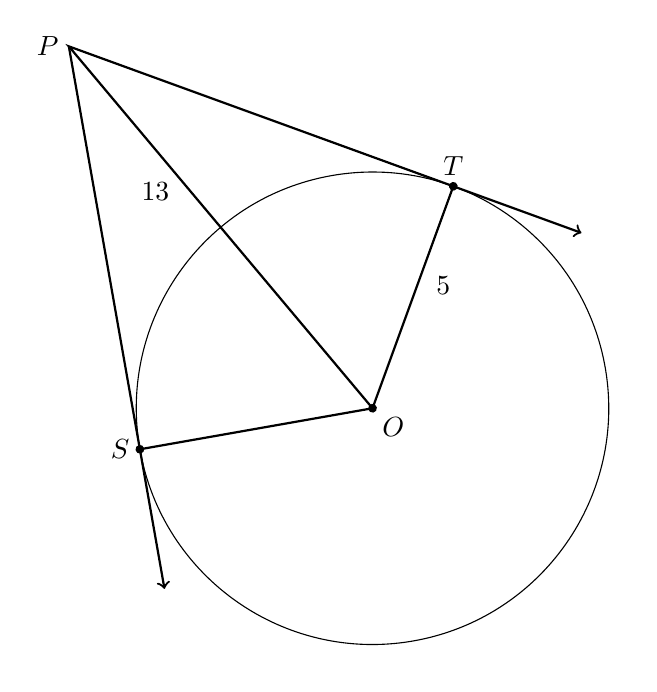
\begin{tikzpicture}[scale=0.6, rotate=-80]
        \draw [<-, thick] (120:5.774)--(210:10)node[left]{$P$}
        --(0,0)--(150:5)node[above]{$T$};
        \draw [->, thick] (210:10)--(0,-5)node[left]{$S$}--(3,-5);
        \draw [thick] (0,0)--(0,-5);
        \draw (0,0) circle [radius=5] node[below right]{$O$};
        %\draw (123:5) ++(-28:0.5)-- ++(-118:0.5)-- +(152:0.5);
        \draw [fill] (0,0) circle [radius=0.08];
        \draw [fill] (150:5) circle [radius=0.08];
        \draw [fill] (0,-5) circle [radius=0.08];
        \node at (215:6.5){13};
        \node at (140:3){5};
      \end{tikzpicture}
   \end{center}\vspace{1cm}

  \item A pyramid with a square base is 8 cm tall, as shown. The slant length, $VM=10$. Find the volume of the pyramid.\\[1cm]
    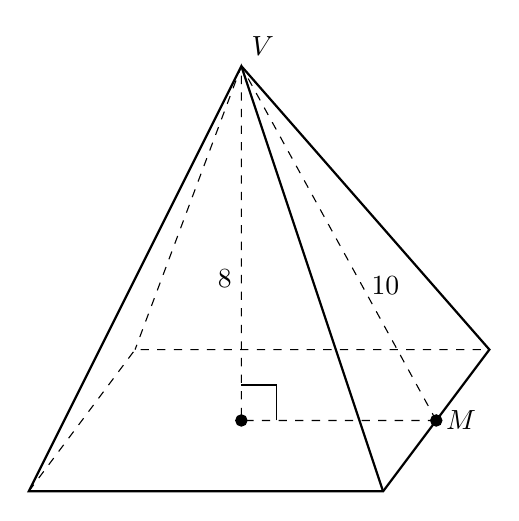
\begin{tikzpicture}[scale=0.9]
      \draw [thick] (-3,-1)--(2,-1)--(3.5,1)--(0,5)node[above right]{$V$}
        --cycle;
      \draw [dashed] (-3,-1)--(-1.5,1)--(3.5,1);
      \draw [thick] (2,-1)--(0,5);
      \draw [dashed] (2.75,0)
        --(0,0)--(0,5)--(-1.5,1);
      \draw (0,0) ++(0:0.5)-- ++(90:0.5)-- +(180:0.5);
      \draw [dashed] (2.75,0)--(0,5);
      \draw [fill] (0,0) circle [radius=0.08];
      \draw [fill] (2.75,0) circle [radius=0.08]node[right]{$M$};
      \node at (0,2)[left]{8};
      \node at (1.7,1.9)[right]{10};
    \end{tikzpicture}

\end{enumerate}
\end{document}
